\subsection{Recommendation in complex software system}
First of all, we have to look at definition of recommendation.  In general, a recommendation is a suggestion or a proposal as to the best course of action, often provided by an authoritative body or expert domain. The key concept when we talk about recommendation is the context, because it changes meaning with respect to the type of system that a developer is working in. 
We can find recommendation system in software engineering (RSSE) that gives the necessary information about suitable items for a software engineering task in a specific context. When a developer starting to work on a project, there are several information spaces, also called landscape, that describe all involved information in the overall developing process. In  ~\cite{martin_p.robillard_introduction_2009}, the authors define all possible information spaces in software engineering but this definition can be applied in whatever software complex system. Related to the developed project, the main definition is the project source code and project history, that give the context of developing. The project source code is useful to understand the structure of it, especially when we looking for method declarations, method calls and possible most frequent pattern while the project history tells something about the changing happened in the code from a older version to another. This changes are usually captured by a VCS (version control system) although this kind of system isn't easily browsable and techniques like data mining or machine learning are required. Development environment also belongs to this information spaces classification and it includes all scripts, commands and tools used to test and run the system. Another big information space is defined by API that are linked to the project as well as their documentation, a good starting point to better understand their behaviours. Moreover, the authors consider also two types of traces when a user is developing a project: interaction traces, composed by the list of user's actions like search on website for particular component or interface and normally this kind of information are captured by an IDE (like Eclipse); the execution trace, instead, regarding the software runtime execution and the collected information are in general function calls and results of computation at every time. Finally, a very important information space is represented by the web that becomes more and more relevant in recent years; in particular, Stack Overflow questions and answers site is the most used by the developers as we can find a lot of concrete example about code snippets as well as information about interfaces, technologies and tools. \newline
As we can see, all this information spaces represent an huge data mine and there are many problems to extract the correct information from it. First of all, the available information are heterogeneous and context awareness while a typical user is looking for a quickly solution related to its specific context. Furthermore, the complex software systems are rapidly growing and it can lead the overload information problem. So, looking at this problem, it is necessary to find a proper way to do recommendation, in the manner that the developer find a good solution in very few time without waste it to search in very large context. For the software engineering context, the authors propose RSSE, a recommendation system for software engineering based on capturing the context, giving the proper recommendation. The process involves some kind of data preprocessing, capturing the context, select the correct recommendation using collaborative filtering techniques and show them to the user. The first phase involves often effort because includes many type of operations on data like transformation, gathering, filtering, aggregation and so on. The next step is the capture of the context, that is a key issue in a recommendation system. In another domains, like e-commerce for example, the context is strongly related to the user's characteristics and its behaviours; reversely, in the software engineering and in the software domain in general, the recommendation are related to the task that the developer wants to perform. So, in this domain we talk about the task context, that in general a smaller part of the final solution. This kind of systems are called task-centric against the human-centric system in which the recommendations are related to the user. However, the capturing of this context could bring some bias, in particular we could be in the situation in which the context are extremely precise, maybe because we have a lot of information, but the user, especially if he is a not expert domain, doesn't known how to use them or how to provide enough information to describe in the proper way the context. After this preparatory phases, a recommendation algorithm can be executed to produce the final output. The literature is plenty of this techniques that go from the collaborative filtering techniques to similarity matrix, as we will see in next section. Of course, the choice of the algorithm to be used affects the precision, the accuracy and the coverage of the approach, making this task the most important during the development of a recommendation system. The last step is the presenting of the recommendation to the final user. Also in this case, the form of representation depends on the domain in which the recommendation system operates; so, considering the context, we can have a list of function calls, variables, classes as well as documentation or issues reports. Beyond the form of recommendations, a recommendation system must be to classify and rank the results, following a well-formed criteria, such as number of lines, probability, time, average rating and so on. This criteria naturally depends once again on the task context. \newline
Moving in the context of the IDEs, auto-completion can be a kind of recommendation at runtime because the developer, usually through shortcuts, wants suggestion for specific functions and methods. This technique uses often documentation embedded in the IDE (like JavaDoc in Eclipse) and it adapts itself  to the context, in this case the imported libraries in the project. Moving to a more general definition, we are in the query auto completion (QAC) domain, used in several contexts like search engine, as described in ~\cite{DBLP:journals/ftir/CaiR16}. It is a particular form of word prediction: when a user is typing something, such as fragment of code,method declaration or just first characters, QAC completes the query using different techniques like n-gram technique, probabilistic methodologies and heuristic learning algorithm. Beyond the used technique, QAC system ranks the possible results of a query following a predefined criteria. In case of auto-completion, the query engine maps the prefix, namely the query that the user is writing, to possible list of results and gather all the date in a effective data structure like prefix tree in order to avoid waste of time. Another purpose of a QAC system is try to predict the user's prefix, by retrieving the top rank queries before the entire process is finished. Moving to the possible approaches, there are two main categories: heuristic model and learning-based model. These two category can be divided again into three categories: time sensitive, contextual based and demographic-based. The first is involved when there are time constrains while the contextual and demographic based categories are strongly related to the user's previous history. \newline
So, we look at the different types of context that a recommendation system must face. Depending on the context, the proposed recommendations change too, sometimes in a radical way. For us, the context are represented by Java projects and in particular, API function call related to external libraries.

\subsection{Learning API: issues and solutions}
Moving on the concept of API, we have also in this case huge amount of definition in the literature and it's necessary to specify very well the context in we are. In general, an API (application programming interface) is defined as a set of procedures, protocols and objects that gives to the developers the necessary building blocks to implement a specific functionality in easy and understandable way. Depending on the context, these building blocks can be classes, interfaces and methods properly declared and used or intermediate software that acts as middleware in different situations as well as in the hardware context. The concept of API is strongly related to libraries that a developer uses and the kind of application that he is developing. So, we can have remote API to interact with different resources like databases deployed anywhere through protocol. An example in Java context is Java Remote Method Protocol. The most famous and used are the web APIs, usually defined in a framework context like MVC or inversion of control. While in the past a web API is associated simply to a web services, nowadays they moving towards SOAP (Simple object access protocol) and REST protocols, as the developers need an easy and quickly usage of the APIs. The basic principle in API development is the information hiding that consists in hide the design principle behind the development of a tool or framework. In this way, when the software needs an upgrade on the functionalities, all the process is done behind the scenes and we will reach a stable interface. \newline
Another issue is the complexity of an API, that depending on different factors like their structure and affect their usability, as pointed out on ~\cite{martin_p._robillard_what_2009}. In this work, the author analyses the developer's difficulties when he wants to approach to an API; in particular, this work looks to the professional developers at Microsoft and try to understand what are the main issues in the API context. As starting point, the author of the article asks to a population composed by 30,000 people among engineers, developers and program manager in the Microsoft context. The survey starts with some questions about the developer's skills, to asses the knowledge of the participants. Then, it contains questions about the problems on learning an API, strongly related to the context, familiarity with the application domain, the obstacles faced during the learning phase and so on. From the initial population, the author select 83 developers and compare the answers between the expert domain, like senior software developer engineering and lead software architects, with the novice and junior developers. From these results, he grouped in five categories obstacles that surface from these people during the learning phase in the API development. Among these, the category with the more answers is the obstacles bring to the absence or inadequate resources in the learning phase, such as not suitable code example, partial information about the content of APIs, no reference about the task to perform, inadequate resources format and insufficient high-level design and not well-formed structure of the API. Other problems are related to the structure, especially for debugging and runtime phases, the developer's background, technical issues and problems that arise during the runtime execution. In order to mitigate these issues, the documentation of an API must include good examples for the functions and code to develop, the support for case study scenarios, good organization of the relevant design elements. Another key point is the context, because the API change often their behaviour depending on it, as pointed out from 12 audio interview that author made with the developers adding their answer to the initial survey. In general, APIs follow the so called low barrier to entry, that consist to give just few information and key concept about the API structure and design, sometimes involving basic code examples. Although it is a very spread techniques, the survey underlines that is not enough to give a concrete help during the learning phase. Many developers involved in the survey, in facts, claim that they are often confused about multiple uses of a certain function, because there are different approaches to implement a feature but they not understand what is the proper one, considering also the context in they are. This issue affects also the general structure of the API, like the design that often generate confusion if it is not well specified and the survey respondents want also to understand what are the rationale behind the API.  \newline
Although the abstract design and the overall structure are important when we talk about the API usage, the most immediate and concrete hints are related to code example, as showed in the proper section of the article that we are analyzing. In particular, the survey shows that the Microsoft developers not always  understand the examples provided in the documentation, as they are not well documented or the authors of API not underline the purpose underlining a particular statement or function. The Table 2 shows the main three category of code example that could be provide by an online documentation or in a general readme file of the API. 
\begin{table}[H]

  \caption{ The three main category of code example }
  \label{Table:2}
\begin{adjustbox}{width=1\textwidth}

\begin{tabular}{|c|p{8cm}|}

\hline
 \textbf{Code example category } & \textbf{Description} \\
\hline
 Code Snippet & It gives just a flavour of basic concepts of the API and their possible use\\
\hline
Tutorial & It is a quite complete example of a possible use of API, with multiple methods and functions usage\\
\hline
Application & It gives a well structured example of the API, given also the development context \\
\hline
\end{tabular}

\end{adjustbox}
\end{table} 

Looking at these categories, the code snippet provides an immediate hint but is more related to a specific issue, such as opening a connection or initialize a particular object. The tutorial provides a more complete examples, with different methods, often followed by a textual explanation with the aim to show the rationale behind the code. The code example coming from the applications, instead, wants to give a general overview on the API features and it includes demonstration samples and complete open source projects. However, the Microsoft developers involved in the survey denote that usually the code snippet doesn't provide how to put together all the small pieces. Another problem is that the code examples on the Internet are out-of-date and the maintenance of them is still an opening question. The author, considering the answers coming from the survey, lists the possible improvements related to the code examples, by providing best practice in a certain situation, by giving the design behind the code example and by showing in a clear way how the API works in practice. All this information should be inserted in the documentation provided with the API. Finally, the author of the survey analyses also the behaviour of an API, that sometime diverges from the declared one in the documentation or from the code examples. The developers suffers in particular for unexpected behaviours of similar components or methods, that varying from a context to another. Although this survey is conducted over Microsoft developers, it points out some key concepts when a user is approaching to learn and use an API, especially for the proper exploitation of provided functions.  \newline
Also in ~\cite{by_christopher_scaffidi_why_2006}, the author underlines some issues and challenges when a developer is approaching to use and understand an API, such as the already mentioned inadequate documentation or the inappropriate abstraction in the overall design. The article suggests also possible workaround for the different situations that the API designers should take into consideration. The ideal design flow when a API designer should be follow includes the gathering of information from the stakeholders (mainly other developers that wants to reuse the API functionalities), map the requested features to the proper components and set up the glue code to make an usable and understandable platform. However, this implies a well specified design flow and a lot of time, and sometimes the timing constrains on the publication of a new API don't allow to have a complete and exhaustive documentation. Also in the case of the Hello World examples, they are often not sufficient for the common user, especially if he is not an expert domain. Another potential problem is represented by the orthogonal functionalities, also called internal couplings. This term refers to the situation in which a method is strongly dependent with another or its behaviour can affect other parts of the system. To avoid these situations, an API's designer must keep the overall platform as simpler as possible, by limiting the exponential growing of the system. Concerning the abstraction problem, the users are in the situation in which the requirements don't match with the proper methods or interfaces provided by the API. This situation go beyond a lack of information in the documentation, because it is a problem that affects the initial design of the API. A designer should set abstractions for each user's requirement, in order to maintain the proper mapping and to avoid the loss of functionalities. Another possible solution is to use the facade pattern to make more accessible the API itself. The last main issue underlined in the article is the external dependencies, called assumptions, that an API could require to perform a certain operation. For the designer a possible solution can be the limitation of external calls to another API, maybe by reusing the internal API features. \newline
All these possible solution that the author provides in the article are inspired by three key concept. The first and most important is to make smaller the problem as possible, by splitting the initial one to little problems that can be solved in less time. Another strategy involves the approximation of the solution, looking first of all to the user's requirements and try to satisfy them. Finally, if the feature or the functionality to implement is really complex, an API's designer should choose an approach that is optimal in the average case. In this way, he reaches good results in reasonable time.\newline
As said before, the usability takes an important role in learning the API. In ~\cite{marco_piccioni_empirical_2013}, the authors focus their attention on this problem, with a human survey similar to the one already analysed. In this case, however, they define two key concept and measure the usability of an API taking into account the so called cognitive dimension and usability token among the participants. The first one involves a cognitive framework based on the human reaction that take place when a user is implementing a particular feature specified by an API. This indicator wants to measure what is expected during the developing and what really happen. With this technique, the authors gather the reactions and so the implicit feedback coming from the programmers avoiding in this way the bias led by subjective perceptions. Of course, the cognitive analysis is combined with the classical research question, about the difficulties to learn a new API, the understandability of the usage and the abstraction of the overall platform. The usability tokens instead are extracted from the interviews to measure different developer's behaviours in different situation. Here below there are the list of the tokens used in the questionnaire:
\begin{itemize}
\item surprise: it measure the unexpected behaviour of a particular component of the API, that seemed different at the beginning;
\item choice: it evaluates the capacity of the developer to understand what is the optimal solution for solving a particular problem, like use the proper data structure;
\item missed: it belongs to the abstraction problem, when the developer loses something because he don't understand the API design;
\item incorrect: in this case, the developer uses in the wrong way the provided function or classes;
\item unexpected: this token describes the situation in which the user takes decisions that are not documented by the API's designer.
\end{itemize}
As we can see, the usability tokens are strongly related with the cognitive dimensions and they can combined with themselves to depict a particular situation in which some obstacles appears at the same time. The experiment is overtaken on ABEL, an object oriented library for storing and retrieving huge amount of information. The results of this empirical study, that involves heterogeneous group of developers, show that the critical issue is to understand the relations between types and classes, not always understand by the participants. Other minors issues are the incorrect usage of the provided interfaces or the treatment of constructors without arguments, but in those cases the developers are able to overshoot these issues. 
So from these works, we can understand the difficulties in approaching an API, as there are many aspects to take into consideration. As we will see, for the our proposed approach we used code example and in particular the snippet of code to perform the recommendation, trying to avoid the above issues related to the API such as the lack of best practices and the ambiguous usage of a component. Another emerging aspect is that the documentation should be clear about the design, the abstraction and the features provides by the API. We don't directly work on the documentation, but we try to offers a solution at level of code that could be integrate this lack of information.



\subsection{Code cloning taxonomy}
To support recommendations, we choose an approach that involves code cloning analysis. When we analyze a software complex system, it is very easy to find duplicated lines of code, especially in case of very big projects. This situation are led by the copy and paste technique, very used in most of situation in which is necessary to save time or simply because it offers an easy solution to the current problem that the developer is facing. Although the copy and paste works in theory, it is not the better solution because the cloned code can bring some unexpected side effects on the other parts of the software and, anyway, it offers a solution only in the short term period. Although this behaviour is discourage in general, many techniques is based on find the clones without removing them. The purpose of these tools, the so called clone cloners, is to analyze software complex system and find the common parts among them. During the analysis, it is also important to clarify how the code has been compared and what the word cloned really means. Two fragments of code could be declared clones also if their are not exact duplicated but even if they share the most of the structure (such as the variable name, the statement structure and method calls). So, a code cloning tool must be analyze also the structure, the AST and the token composition, plus the textual plain code of course. There are several techniques in the code cloning field and we look at ~\cite{chanchal_k._roy_comparison_2009} to have a brief but clear overview on this topic. In general, a clone detector try to find the similarities between two fragment of source code. These analysis depend first of all from the level of details that the tool wants to reach: to make a very simple example, each code cloner could be set a different similarity function in order to set the level of cloning. They differs also in term of the comparison of two fragment of code, such as AST, textual comparison and so on. As we can see, there are a lot of concepts and techniques in this approach and to avoid get confusing, the authors create a very useful taxonomy to classify the activity of code cloning, showed in table 2.

\begin{table}[H]
 \caption{ Code cloner tools taxonomy}
 \label{Table:2}
\begin{adjustbox}{width=1\textwidth}
\begin{tabular}{|p{3cm}|l|}
\hline
\textbf{Code cloner type} & \textbf{Level of similarity}  \\
\hline
Type-1 & The code fragments differs only from the whitespaces, comments ad layout \\
\hline
Type-2 &  \vtop{\hbox{\strut Two code fragments that are syntactically equals}\hbox{\strut  except for the same conditions of type-1 plus identifiers, literals and name variables   }} \\
\hline
Type-3 &  \vtop{\hbox{\strut This kind of clone detector looks for variation (add, delete or change) in statement}\hbox{\strut that appears in the fragments, plus the previous conditions  }} \\  
\hline
Type-4 &  \vtop{\hbox{\strut We have this kind of cloner when the computation that the fragments}\hbox{\strut perform are equal without considering the syntactic implementation   }} \\
\hline



\end{tabular}

\end{adjustbox}
\end{table} 


Although there are a huge number of tools and techniques, there is a common clone detection process that it has to be considered in order to avoid very critical loss in time and spaces. In fact, even using whatever tool the computation became a big issue if the common part among fragments are unknown at the beginning of the process. So, the authors identify an overall process to approach the code cloning activity, even all the steps are not required depending on the situations. The preprocessing phase, first step, is necessary to discard useless elements in the fragments of code like embedded code that appears in some language and to obtain the source units. These units can be very different depending on the purpose of the cloner and sometime they can be partitioned again in comparison units, depending on the structure of the original source unit (the common case is when we have an if-else structure in which the comparison units could be the different branches). After the preprocessing, if the code cloner go further the textual analysis, a transformation phase is required, to bring all the fragments to a common representation. Among the possible normalizations that we can apply to code fragments, we have the removal of whitespaces and comments, the normalization of identifiers (for example, through order sensitive index scheme), pretty-printing that affect the layout and structural transformation (for example, by removing the modifiers in a particular language). When we have a comparable units, a different comparison algorithm is run depending on the tool in order to obtain the list of matches. In this phase, we have to distinguish the fixed-granularity tools, in which the units that belongs to same block have the same granularity from the free-granularity ones in which the aggregation continues until a threshold value is reached. The list of candidates for the comparison are usually source coordinates that must be map on the original source code files. The last step is a post-processing in which clones are ranked or filtered depending on the aim that the tool wants to reach. This phase can be done by human evaluator or through a parametric heuristic algorithm. The picture below summarizes the entire procedure:\\

\begin{figure}
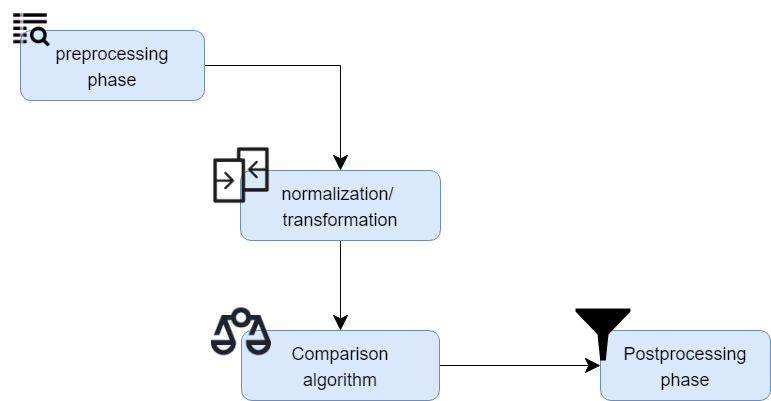
\includegraphics[width=14cm,height=14cm,keepaspectratio]{images/codeCloning.png}
\centering
\caption{Typical code cloning phase}
\label{fig:cmd}
\end{figure}

Looking now to the different tools, most of them rely on different approaches to identify cloned code. The most immediate approach is the textual one, as the transformation and normalization phases are often very slight. The tools that implement this approach use fingerprints or substring of the source code. The fixed lines that are used in the comparison are called window and they are encoded with a hash function. To obtain fragments with different lengths, the tool apply simply a slicing on the window. The lexical approach, instead, works on the tokens obtained from the source code through the compiler-style lexical analysis. This technique is more robust because it avoid the whitespaces and other dirty code that we want to exclude from the comparison. The big issue of this approach is that it not consider the syntax; so, the founded clones may overlap different syntax units but preprocessing or postprocessing can avoid this situation, like pretty-printing techniques to format the code in a better way. Go further, we now look at the syntactic approaches, that usually rely on the AST of the code. There are two main process  that we can apply: the tree matches and structural metrics. The first relies only on the AST extracted from the code and the comparison takes place on the subtrees. Each element of the source code(variables, literals) became a leaf of the tree and subtrees that are hashed into buckets in order to reduce the number of comparisons that take place in each bucket. However, the complexity of this approach is very high and recently there are code cloner that try to mitigate this drawback by serialize the AST as node sequence in order to reach the same speed in the same way of  token based techniques. The second approach  exploits the AST is based on structural metrics. This technique avoid the direct comparison between ASTs by collecting a vector of metrics, usually calculated through fingerprints functions that consider classes, methods and statements for the metrics. The last approach that we look is the semantic technique that relies on static program analysis to provide more information rather than the syntactic one. With respect to the other approaches, the source code is represented by a PDG (Program Dependencies Graph) to keep trace the data dependencies among expression and statements. So in this case, the comparison of the clones turns to the problem of finding isomorphic subgraphs. Finally, in the literature we can find hybrid approaches that involves both syntactic and semantic analysis. \\
This work includes also a very useful tool comparison, in which the authors show a list of code cloners and their main features. This state of the art is done by taking into account several parameters and metrics, like availability of the tool, IDE integration, comparison algorithm, kind of granularity, pre or post processing, language support, subsystem, possible empirical validation and overall complexity. However, it is not easy to evaluate code cloning tools, because there are several factors and hypothesis to taking into account when we do the comparison. As we have seen, each code cloner have its own techniques, comparison algorithm, approaches, complexity and supported languages, so the risk to do an unfair comparison is concrete. To avoid this situation, the authors set a list of possible scenario that analyze different kind of situations in which the code cloning activity may be useful. The evaluation analyzes the results and if the considered code cloners are able to detects the common part in particular duplicated snippet of code. There are two type of scenario that the authors consider in the evaluation: the first type is more technical and it considers the changes at the level of code, taking as example functions that implements some features. The second type of scenario involves more a not expert domain user and it focuses on the intentions rather than directly on the features. For the first type of scenario, we have several functions that implement a very simple mathematical operation. By the copy and paste activity in which literals, variables and statement change from one scenario to another, the authors look for the code cloners that are able to detects these changes. Some scenarios also take into account the changes that happening in the code like addition or deletion of lines of code. In the second scenario, instead, a user claims the functionality that he wants to realize or how many clones in the code the cloner found. 
\newline
\subsection{Code cloners: techniques and features}
After the code cloning taxonomy, useful to give a general but exhaustive idea about the code cloning domain, we show some code cloners that use interesting techniques to solve the problem of first track the cloned code and thus retrieve the results to the developer. Among the these techniques, we are focusing on the string match one, as it is closer to the code snippets used in our approach. The detection of cloned code is a complex task, that can be bring different issues and criticisms. As pointed out on ~\cite{stephane_ducasse_effectiveness_2005}, there are key points to take into account we are looking at the string match code cloner. First of all, it is necessary to avoid false positive, the part of code that is marked as duplicated but should not be, and false negatives, that appears when the code cloner is not able to detect the cloned code during the analysis. Moreover, the scalability takes an important role in this task, because the code cloning tool must analyse complex software system that are exponentially growing in recent years. An strongly related issue is also the analysis of multiple languages: a good code cloner, in facts, should be able to recognize the cloned code beyond the different syntaxes and lexical differences among the different programming languages. Then, the authors propose their approach, based on the lexical analysis, following the Bellon's case study about the code cloning. In this framework, the author categorizes the clones into three types: the exact clones (Type 1), the part of code that differs from each other for the identifiers (Type 2) and clones in which statements or expressions have been inserted, deleted or changed (Type 3). This case study provides also a measure to detect how a clone is far from an other, in term of the distance. Before proceeding with the tracking activity, the authors make also the so called noise elimination on the source files that contain the cloned part to find. The noise elimination, according to the implementation done by the authors of the article, is similar to the token normalization mentioned in the taxonomy part: they remove all black spaces, comments and blocks that are not useful for the comparison. This phase is necessary to avoid false negative. Once they have done this normalization, they can apply the string matching techniques, based on a line by line comparison in which they look for duplicated code. From their experience, it is very difficult to find an exact code, following the definition of the Bellon'work; it is most probable to find the duplicated code among the code fragments with some modification, like insertion or deletion of statement, variable and so on. Finally, the apply some filters on the results, as the single line is not enough to be significant for the cloning analysis. Therefore, they set two metrics, one related to minimum length sequence of the duplicated part, and the second related to the maximum gap size, measured between two compared sequences. To improve the recall of the results, they also set up a second normalization based on regular expression and they test the overall approach on the same dataset of Bellon's study, composed by the Cook and Weltab application. 
\\
Another interesting approach for the code cloning is showed in ~\cite{nils_gode_incremental_2008}, in which the author proposes a code cloner with multiple revision of the code. In this way, the analysis takes place not only on the original code but also on the fragments already processed, in order to give a more accurate analysis. For this purpose, he develops the IDA tool (Incremental detection algorithm). It is based on tokens, a sequence of characters with a collective semantic, and on suffix trees, already mentioned before. In particular, for the token the author use a multiple token table as data structure, in order to avoid the problems that arise during the multiple revision task. In facts, during the analysis tokens already analyzed by the tool must be discarded from the next phases and this could be left holes in the table, with a consequent overhead in the basic operations like the access to data. So, when a new fragment of code is analyzed, a related token table has been created to speed up the operation. Also the suffix tree is affected by these side effect and the IDA tool uses a generalized suffix tree to solve these issues. In this version, the suffix tree has multiple strings instead of one. The main advantage is the speed of the operations like deletion or update of a single leaf. Similar to the token tables, the fragment of code already analyzed is deleted from the tree. Considering also the clone pairs, IDA integrates all these components in order to make the multiple revision of code. The process starts with a preprocessing phase in which IDA sets up the necessary data structure in and reads the source files from the directory. Once this initial phase ends, the tool starts to build the token tables and the corresponding edges and nodes in the suffix trees when it is processing new files; reversely, it deletes the nodes of external edges that represents the deleted files. The approach is tested on three open source software, wget for downloading files, gcc compilers and the Linux kernel. \\
The last example that we show is related to Cren  ~\cite{jablonski_cren:_2007}, a code cloner specifically developed for IDEs. In particular, the author set up our tool for Eclipse platform, going further with respect to the related Eclipse features, like refactor or  find and replace. The issues to face in this field are mainly related to copy and paste that the a typical user do to integrate into an IDE another methods or function. Reversely with respect with other approaches, that use heuristic algorithms often very complex, the authors of Cren provide a simpler but  effective solution in the IDEs context. The core of the approach is represented by a tracking of cloned part, followed by consistent rename of variables, that is the typical behaviour of a developer when he tries to reimplement an API component. By exploiting the JDT features related to the AST of the code, Cren is able to find not only the cloned pairs but also a clone groups, represented by a sequence of two or more elements. Variables and identifiers that share some characteristics are inserted in a same group. Once it found the clones, it can show to the user what are the cloned part in the context and, thanks to Eclipse interface, it is able to highlight the cloned pairs that change dynamically with respect to the context. In this way, the user can refine also the search of the cloned parts, as Cren keeps trace about the cloned part already founded. Cren represents an interesting mix between the code cloning technique and the IDE context. After this overview about the taxonomy of code cloning and some examples of code cloner, focused in particular about the suffix tree technique and an incremental code cloner, we will see in the next section the code cloner chosen for the implementation of our proposed approach. 
\newpage
\subsection{Simian overview}
As we see from the introduction, we can perform recommendation at different levels of abstraction (pattern, documentation, code snippets) in order to give a complete and useful hints to a developer. In our approach, the overall idea is to perform the API recommendation at the level of code snippets that represent the patterns related to the developer's file. To do this, we can exploit the code cloning analysis that we present in the previous section. As tool for this approach, we choose Simian, a project developed in Java that performs this kind of analysis for many languages as Java, C, C\#, Ruby, JavaScript, COBOL, Lisp, SQL, Visual Basic. Following the taxonomy in table 2, we can define Simian as a Type-2 code cloner with flexible options on variables, literals, modifiers and it performs the analysis following the textual approach described before. All possible options are described in table 3, although we discard some options that are related to languages different from Java, like ignoreRegions for C files. To test the main functionalities of the tool, we can simply run the jar file a available on the website   ~\cite{https://www.harukizaemon.com/simian/_last_nodate} by specifying options and the input file. As output, we see on the console the textual representation of source coordinates that describe the number of duplicated lines and the original source files. The results are showed on the console. Notice that we can change the type of output using the formatter option (in table 3). 
Following the tool classification already mentioned, Simian has this following features: 
\begin{itemize}
\item It supports object oriented and web languages;
\item It not require additional tools or dependencies;
\item It is language and platform independent;
\item It has free granularity and it analyze line by line of the source files;
\item It uses fingerprints technique for the code representation;
\item It applies transformation on variable, types and literals using options.
\end{itemize}
Among the main drawbacks, Simian not include IDE supports and we must do a manual integration that we will see in next section. Moreover, it not includes some preprocessing or postprocessing phases as well as an heuristic algorithm for the threshold or an aggregation phase at the end of the process. It has no external dependencies and it is free downloadable but empirical evaluation is not available. Also the algorithm complexity is not well define, although it depends first of all by the number of lines of code and on the website there is a time approximation for one comparison. In particular, Simian is able to find 141,070 duplicate lines of code in 2,406 files in less than 5 seconds, that means about 28 lines of code for each second. 



Table4 describe a very simple scenario in which we pick four pairs of Java project with the description of their main features and how lines of code are in commons.

\begin{center}
\begin{table}[H]
  \caption{ Simian options used in the experiment }
  \label{Table:3}
\begin{adjustbox}{width=1\textwidth}
\small
\begin{tabular}{|l|p{4cm}|p{6cm}|}

\hline

 \textbf{Option name} & \textbf{Default value} & \textbf{Description} \\
\hline
 -threshold & 6 &This option fix an lower bound on the number   of duplicated lines of code (if present)  \\
\hline
-formatter &  none , possible values: plain, xml, emacs,    vs (visual studio), yaml, null &   This option is used to obtain results in a specified format\\
\hline
-reportDuplicateText & disable , type + to add &   With this option, the duplicated lines of code  present in all projects are printed on the console    \\
\hline
-language & disable , type + to add &  This option specify the  language of the input files to compare   \\
\hline
-defaultLanguage & disable , type + to add &   If not file type is not specified, Simian inferred the type and set it as default    \\
\hline
-failOnDuplication & able , type - to remove & If this option is able, it causes  an exception when the checker finds duplicate code     \\
\hline
-reportDuplicateText & disable , type + to add & With this option, the duplicated lines of codepresent in all projects are printed on the console    \\
\hline
-ignoreRegions & disable , type + to add & It ignores block in regions structures (only for C\# programming language)  \\
\hline
-ignoreBlocks & disable , type + to add &  It excludes specified blocks  from the comparison (start/end line must be specified  \\
\hline
-ignoreCurlyBraces & disable , type + to add & The curly braces are ignored  so it should be match as duplicate line \\

\hline
-ignoreIndentifier & disable , type + to add &   With this option, the variable with different identifiers match as equal  \\
\hline
-ignoreIdentifierCase & able, type - to disable &  This option not consider the case of identifiers  present in the code: so Name and name are considered equal \\
\hline
-ignoreStrings & disable , type + to able &  This option consider all strings  in the comparison and  doesn't take care about the form in which are write\\
\hline
-ignoreStringCase & able, type - to disable & Same as previous option   but consider the upper and lower case as the same \\
\hline
-ignoreNumbers & disable, type + to add &   This option considers different    numbers as equal  \\
\hline
-ignoreCharacter & disable, type + to add &    With this option, all character type match as equal  \\
\hline
-ignoreCharacterCase & able, type - to disable &  Same as ignoreStringCase but consider char by char. Useful for more precise analysis \\
\hline
-ignoreLiterals & disable, type + to add &   All literals should be seen  as equal for Simian  \\
\hline
-ignoreVariableNames & disable, type + to add &   This option allow to Simian  to see different variable names as equal \\
\hline
-ignoreModifiers & able, type - to disable &   This option doesn't consider modifiers of methods  (public, private, protected as element of  diversity in the code)\\
\hline



\end{tabular}

\end{adjustbox}
\end{table} 
\end{center}



\begin{center}
\begin{table}[H]
  \caption{ Projects considered in the comparison }
  \label{Table:4}
\begin{adjustbox}{width=1\textwidth}
\small
\begin{tabular}{|l|p{5cm}|p{3cm}|}

\hline
 \textbf{Projects name} &  \textbf{Main features}  & \textbf{Similarity level (duplicated LOC)}  \\
\hline
 ADTPlugin, ModiscoPlugin   &  Plugin projects created with same wizard & 39 lines of code in common\\
\hline
CyberGea, NeoEMFExample &   Very different projects that realize different features & No lines in common\\
\hline
CyberGea, Scuna project & The projects share only database part & 12 lines on common  \\
\hline
Simple Servlet, ServletSession &  Web projects with servelts & 35 lines of code in common  \\
\hline
\end{tabular}

\end{adjustbox}
\end{table} 
\end{center}

From the scenario, we can see that similar project share more line of code, like the first two pairs that are both Eclipse plugin projects. It happened because these projects are built with the same wizard procedure and share the initialization phase of the plugin, such as the activate method. The second pair of projects, instead, doesn't share any lines because the CyberGea project is another plugin projects that uses Mqtt paho client and JDBC libraries mainly while the Neo EMF project is related to construct a metamodel with the aim to create a Neo4j database. Then, we compare Cybergea with another project developed in this university, the Scuna project that involves Swing framework and the MySql library for java. Notice that in this case, the two project shares only this latter part and the lines in commons are very few. The last example is related to Java Servlet in the web context and Simian analyze two kind of servlet, one without the handling of session and the second with this features. The tool is able to detect that there are many lines in common, as the servlet shares the initialization part in commons like the doGet and doPost methods. Notice that all the projects showed in this simple comparison are developer in the context of university projects and their aim here is only to show an example of the code cloning activity of Simian. As an additional remark, for this comparison we use the default options for Simian and launch it from the console, again just to give the taste of the kind of analysis that we will perform at deeper level for the proposed approach. \\ 
Before to go in deep in the explanation of our approach, we present now existing approaches that face the problem of API recommendations, considering different techniques and contexts.